  
\documentclass[letterpaper, 12 pt]{article}
\usepackage{indentfirst}
\usepackage{color}
\usepackage{hyperref}
\usepackage{graphicx}
\usepackage[portuguese]{babel}
\hypersetup{
    colorlinks,
    linktoc=all,
    citecolor=black,
    filecolor=black,
    linkcolor=black,
    urlcolor=black
}


\renewcommand{\contentsname}{Sumário}

% -------------------------------------------------------------------------------------
% BEGIN DOCUMENT
% -------------------------------------------------------------------------------------
\begin{document}
\title{Manual de Utilização do Sistema de Controle de Estoque Bloco K}
\author{Departamento de Tecnologia da Informação - CECRF}
\maketitle
\pagestyle{empty}
\newpage


% -------------------------------------------------------------------------------------
% TABLE OF CONTENTS
% -------------------------------------------------------------------------------------
\tableofcontents
\newpage

% -------------------------------------------------------------------------------------
% INTRODUCTION
% -------------------------------------------------------------------------------------
\section{Introdução}
Sistema desenvolvido para controlar e rastrear os insumos recebidos pelo Centro de Radiofarmácia.
\newpage


\section{Acesso ao sistema}
Para seu desenvolvimento, foi utilizado como navegador padrão o Google Chrome, mas o software pode ser utilizado 
no Mozila Firefox e Microsoft Edge. Preferencialmente a indicação é o navegador do Google.
\subsection{URL de acesso}
Digite no navegador o seguinte endereço: http://10.0.4.7:8080/www
\subsection{Login}
A seguinte página, Fig. \ref{figura:login1}, deve abrir após o acesso pela URL. Uma vez logado, o sistema grava num token as credenciais (email e senha), onde fica armazenado por 24 horas, sendo desnecessário novo login neste espaço de tempo.
O novo usuário deve se cadastrar clicando no botão registrar. Se o usuário ja está cadastrado mas não lembra a senha só clicar no botão esqueci a senha e informar o email que o software envia uma nova senha.

\begin{figure}[h]
\centering % centralizar figura
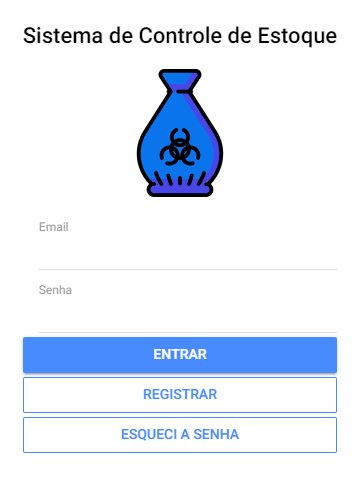
\includegraphics[width=5cm]{imagens/login1.PNG}
\caption{Tela inicial de login}
\label{figura:login1}
\end{figure}
\newpage

\subsection{Registrar - Novo Usuário}
Na  Fig. \ref{figura:registrar1} temos o formulário de cadastro de um novo usuário. Os campos com asterisco são obrigatórios, e o email inserido deve ser válido e será utilizado como login de acesso. 

\begin{figure}[h]
\centering % centralizar figura
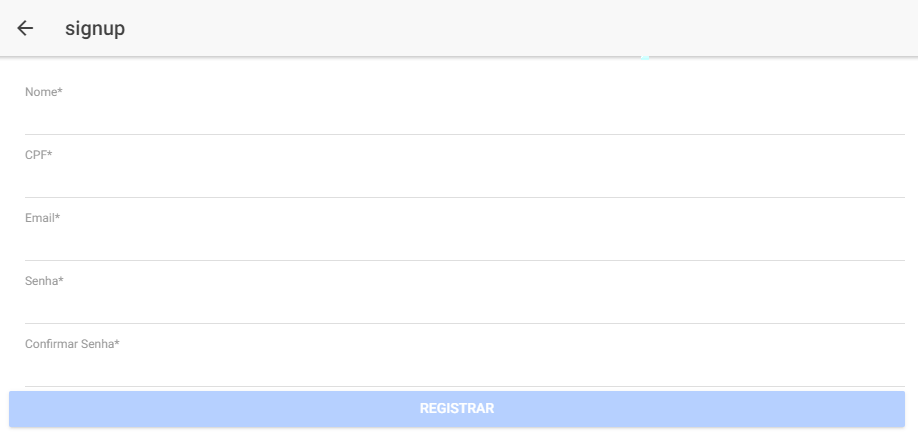
\includegraphics[width=10cm]{imagens/registrar1.PNG}
\caption{Registro de novo usuário}
\label{figura:registrar1}
\end{figure}

\subsection{Esqueci a Senha}
Na  Fig. \ref{figura:recuperar1} temos o formulário de recuperação de senha. Apenas inserir o email cadastrado e o software envia uma nova senha para o email informado. Após isso a senha poderá ser trocada pelo menu Profile.

\begin{figure}[h]
\centering % centralizar figura
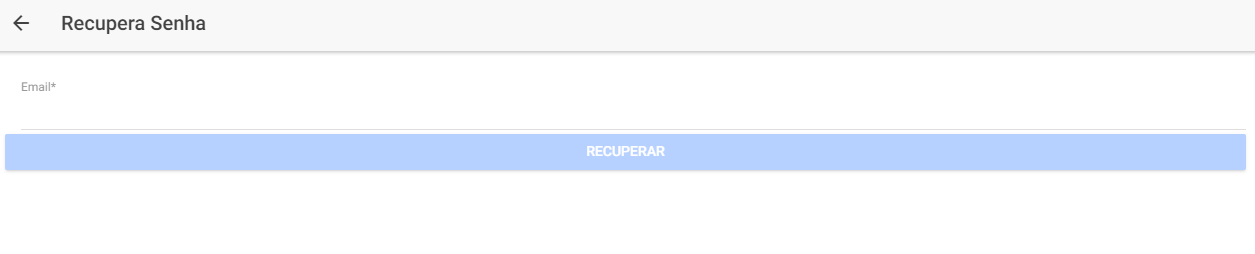
\includegraphics[width=10cm]{imagens/recuperar1.PNG}
\caption{Recuperação de senha}
\label{figura:recuperar1}
\end{figure}
\newpage

\section{Software}
Após logado, o sistema redireciona para a tela principal, Fig. \ref{figura:dashboard1}, identificada como Dashboard, trazendo informações relevantes sobre o estado atual de insumos no banco de dados. Ao lado do nome Dashboard podemos acessar o menu onde contem todos os links para as páginas do sistema, Fig. \ref{figura:menu1}.

\begin{figure}[h]
\centering % centralizar figura
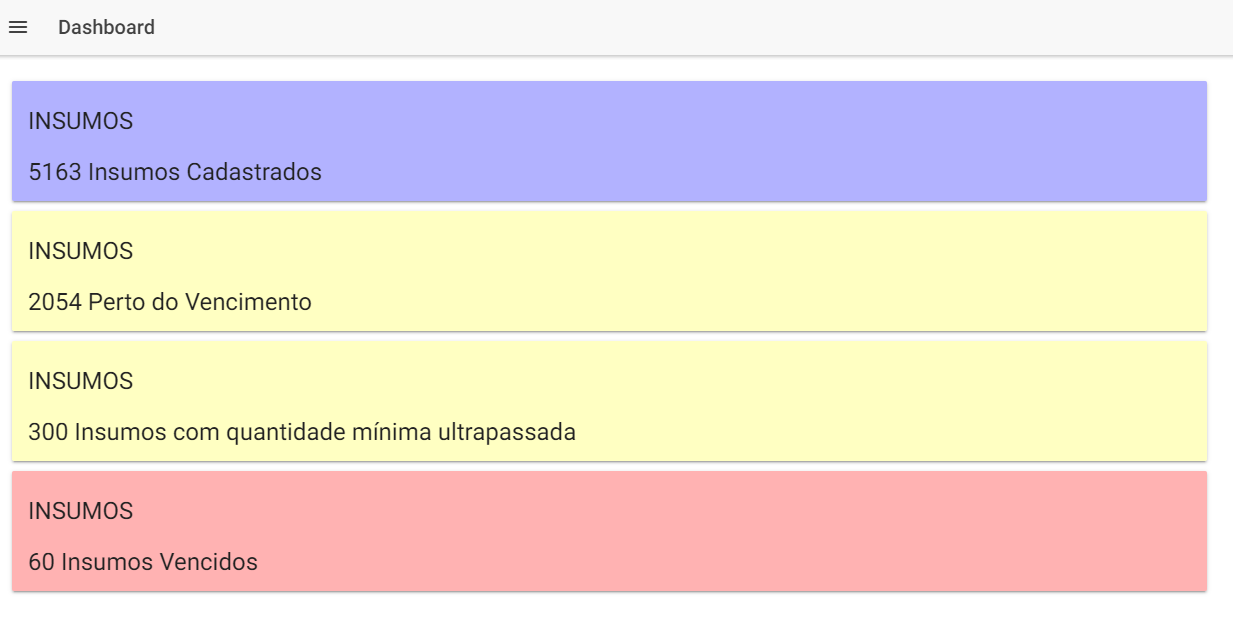
\includegraphics[width=9cm, height=4cm]{imagens/dashboard1.PNG} 
\caption{Tela inicial do software}
\label{figura:dashboard1}
\end{figure}

\subsection{Menu do Software}
Neste momento, podemos acessar todas as páginas do software. Abaixo uma breve descrição de cada link:

\begin{itemize}
  \item Dashboard: Métricas de insumos;
  \item Produção: Em desenvolvimento;
  \item Insumos: Listagem e cadastro de insumos;
  \item Produtos: Em desenvolvimento; 
  \item Categorias: Listagem e cadastro de categorias;
  \item Fornecedores: Listagem e cadastro de fornecedores;
  \item Unidades de Medida: Listagem e cadastro de unidades de medidas;
  \item Localizações: Listagem e cadastro de localizações; Insumos por localização;
  \item Movimentações: Listagem e cadastro de movimentações;
  \item Entradas: Listagem e cadastro de entradas;
  \item Saídas: Em desenvolvimento;
  \item Profile: Usuário e alteração de senha;
  \item Logout: Sair do sistema.
\end{itemize}

\begin{figure}[h]
\centering % centralizar figura
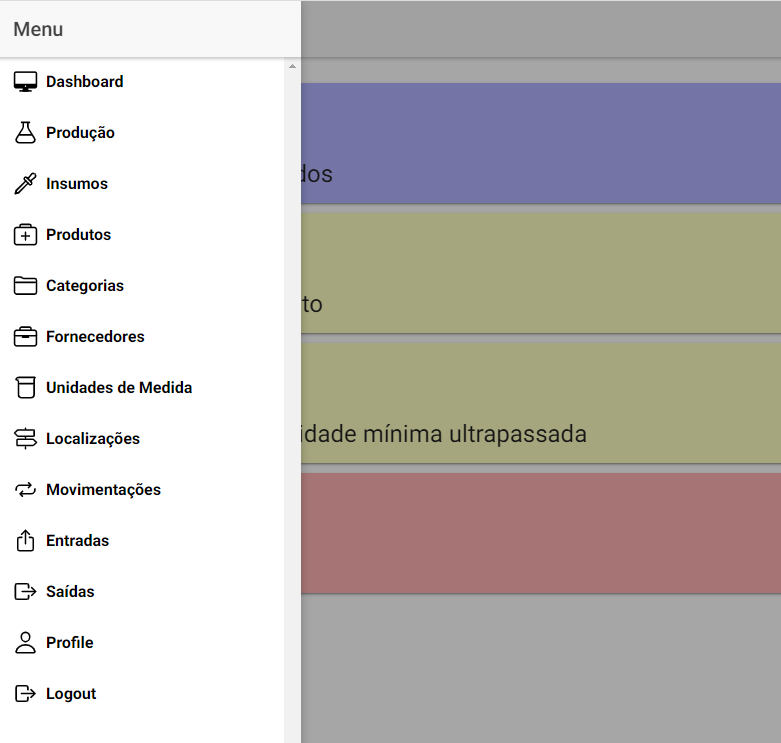
\includegraphics[height=6cm]{imagens/menu1.PNG} 
\caption{Tela inicial do software}
\label{figura:menu1}
\end{figure}

\subsubsection{Dashboard}
Traz um resumo da situação dos insumos no banco. 

\subsubsection{Produção}
Em desenvolvimento.
\newpage

\subsubsection{Insumos}
Nesta tela, Fig. \ref{figura:insumo1}, podemos visualizar todos os insumos cadastrados no sistema bem como cadastrar um novo insumo, Fig. \ref{figura:insumocadastro1}, clicando no sinal de + no canto superior direito.

\begin{figure}[h]
\centering % centralizar figura
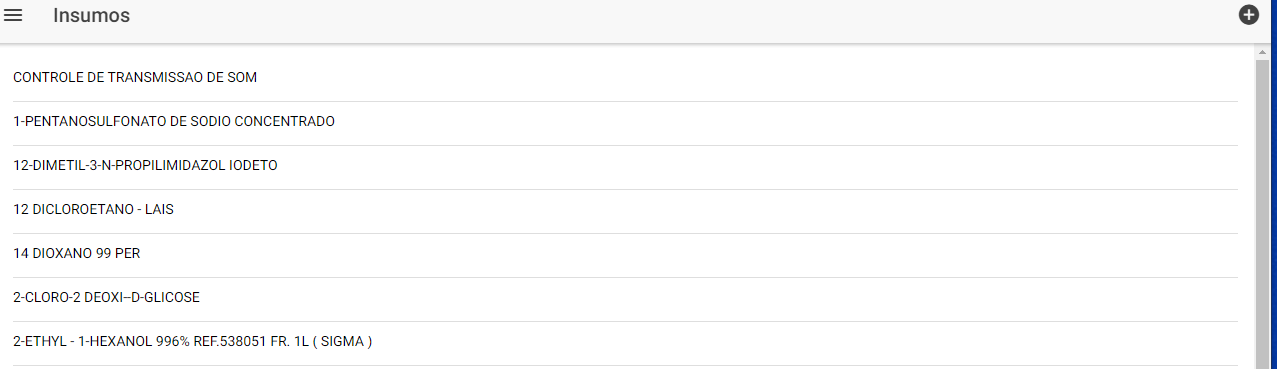
\includegraphics[width=14cm]{imagens/insumo1.PNG} 
\caption{Tela de listagem de insumos}
\label{figura:insumo1}
\end{figure}

\begin{figure}[h]
\centering % centralizar figura
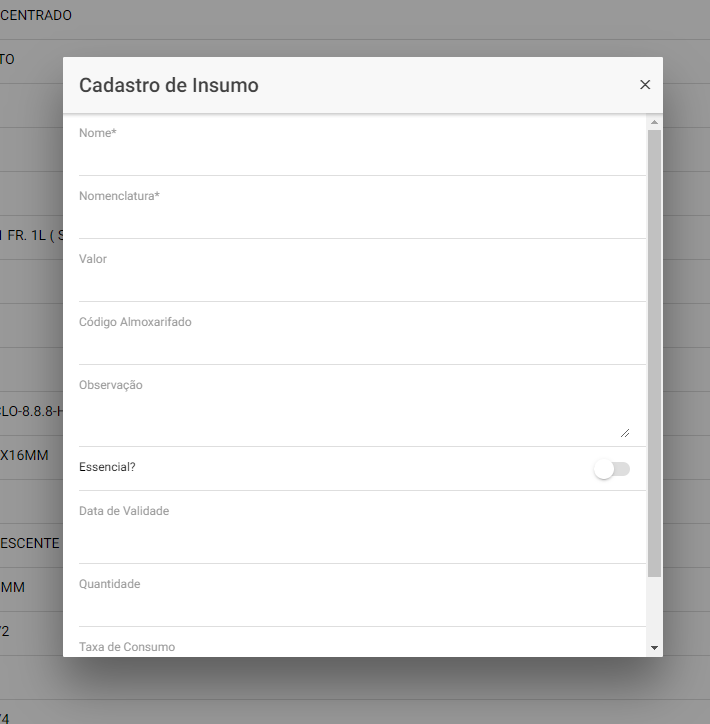
\includegraphics[height=8cm]{imagens/insumocadastro1.PNG} 
\caption{Tela de cadastro de insumos}
\label{figura:insumocadastro1}
\end{figure}
% -------------------------------------------------------------------------------------
% REFERENCES
% -------------------------------------------------------------------------------------
%\bibliography{}

% -------------------------------------------------------------------------------------
% END DOCUMENT
% -------------------------------------------------------------------------------------
\end{document}